\documentclass[conference]{IEEEtran}
% \IEEEoverridecommandlockouts
% The preceding line is only needed to identify funding in the first footnote. If that is unneeded, please comment it out.
\usepackage{cite}
\usepackage{amsmath,amssymb,amsfonts}
\usepackage{algorithmic}
\usepackage{graphicx}
\usepackage{textcomp}
\usepackage{xcolor}
\def\BibTeX{{\rm B\kern-.05em{\sc i\kern-.025em b}\kern-.08em
    T\kern-.1667em\lower.7ex\hbox{E}\kern-.125emX}}
\begin{document}

\title{Impacts of Hyper-Parameter Tuning on Facial Recognition Bias in Computer Vision\\
% {\footnotesize \textsuperscript{*}Note: Sub-titles are not captured in Xplore and
% should not be used}
% \thanks{Identify applicable funding agency here. If none, delete this.}
}

\author{\IEEEauthorblockN{Ghaida Al-Atoum}
\IEEEauthorblockA{\textit{Lyle School of Engineering} \\
\textit{Southern Methodist University}\\
Dallas, TX USA \\}
\and
\IEEEauthorblockN{Wilma Davis}
\IEEEauthorblockA{\textit{Lyle School of Engineering} \\
\textit{Southern Methodist University}\\
Dallas, TX USA \\}
\and
\IEEEauthorblockN{Christopher Henderson}
\IEEEauthorblockA{\textit{Lyle School of Engineering} \\
\textit{Southern Methodist University}\\
Dallas, TX USA \\}
\and
\IEEEauthorblockN{Tango Tew}
\IEEEauthorblockA{\textit{Lyle School of Engineering} \\
\textit{Southern Methodist University}\\
Dallas, TX USA \\}
}

\maketitle

\begin{abstract}
The increasing application of computer vision in facial recognition technology has raised concerns about racial bias. Prominent deep learning architectures, such as ResNet and VGG, dominate this field. A review of existing research reveals a lack of in-depth exploration into how selected or built-in hyper-parameters affect the performance of these algorithms in addressing racial disparities. This paper delves into the implications of hyper-parameter tuning and its potential to alter facial recognition outcomes.
\end{abstract}

\section{Motivation}
As advancements in computer vision increase, the application of facial recognition becomes more important. Today, a multitude of use cases impact our daily lives. Decisions involving employment, public security, criminal justice, law enforcement surveillance, airport passenger screening, and credit reporting \cite{labati2016biometric,amos2016openface} are just a few examples. The importance then, of understanding the underlying drivers of racial bias contributors is imperative to ensuring racial equity is present in them. We present several examples supporting the claim that the composition of data in many datasets are a contributing factor to racial bias. 

Joy Buolamwini and Timnit Gebru in their seminal paper \textit{Gender Shades}\cite{pmlr-v81-buolamwini18a}, found that "a demographic group that is underrepresented [e.g. Black Females] in benchmark datasets can nonetheless be subjected to frequent targeting." Their study automated face recognition by law enforcement further illustrates the need for improvement. "A year-long research investigation across 100 police departments revealed that African-American individuals are more likely to be stopped by law enforcement and be subjected to face recognition searches than individuals of other ethnicities. False positives and unwarranted searches pose a threat to civil liberties. Some face recognition systems have been shown to misidentify people of color, women, and young people at high rates." Another example, Thomas Hellstrom, Virginia Dignum and Suna Bensch describes COMPAS, a computer program used for bail and sentencing decisions "has been labeled biased against black defendants\cite{hellstrom2020bias}."

Examples of such partiality abound. Nada Hassanin quotes faculty of Law assistant professor Dr. Gideon Christian at the University of Calgary in her article \cite{Hassanin_2023}, “technology has been shown to have the capacity to replicate human bias. In some facial recognition technology, there is over 99\% accuracy rate in recognizing white male faces. But, when it comes to recognizing faces of color, especially the faces of Black women, the technology seems to manifest its highest error rate, which is about 35 per cent.”

In this paper, we intend to explore methods inspired by \cite{maze2018iarpa} and conduct analysis to determine whether the effects of hyper-parameter tuning on neural network architectures could potentially decrease some of the large error rate gaps identified in most facial recognition systems. 

Through this investigation we seek to answer the following research questions:
\begin{enumerate}
    \item How do specific hyper-parameters influence racial biases in facial recognition, particularly across different racial groups?
    \item Can modifications in the kernel size of a convolutional neural network (CNN) improve the detection of facial features across diverse racial groups, thus reducing bias?
    \item Does increasing the depth (number of convolutional layers) of a CNN by adding more layers affect the racial bias error rates?
\end{enumerate}

Further, we hypothesize that strategic adjustments in hyper-parameters, such as kernel size and the number of convolutional layers, can significantly influence the performance of facial recognition systems, potentially reducing racial bias.

\section{Related Work}
\cite{yucer2023racial} Surveys all papers written until May of 2023 regarding racial bias within face recognition and efforts to mitigate it at each stage of the pipeline. Various means exist by which bias enters facial recognition models. Acquisition, the stages of initial image pre-processing and formulation from online resources which could introduce sampling bias; Face Localization, a facial alignment step to correct for positional, rotational, and scale variations of obtaining a canonical facial image representation which could be affected by pose bias; Face Representation, the process of optimizing a model to embed images into a feature embedding space and could introduce hyper-parameter bias and uncertainty bias; Face Verification, which includes one-to-one matching to determine whether two images belong to the same individual; and Face Identification, the one-to-many matching operation to identify an individual against  a set of reference images, both of which may introduce evaluation bias when the dataset used to evaluate is not accurately representative of the target population \cite{suresh2021framework}.

Buolamwini and Gebru present the evaluation of three commercially available gender classification systems from Microsoft, IBM, and Face++ in\cite{pmlr-v81-buolamwini18a} and finds that darker-skinned females are the most misclassified group. Error rates among darker-skinned females reached a maximum of 34.7\% while similar rates for lighter-skinned males was 0.8\%. The authors developed a custom face image dataset called Pilot Parliamentary Benchmark (PPB) composed of images of members of parliament from three African countries and three European countries. They introduce the first intersectional demographic and phenotypic evaluation of face-based gender classification accuracy using the Fitzpatrick skin types\cite{fitzpatrick1988validity}, to their knowledge the first gender classification benchmark to do so. 

Concepts that comprise good facial recognition datasets are introduced in \cite{monnerat2007machine} including technical standards International Organization for Standardization/International Electrotechnical Commission (IOS/IEC) 19794-5 and International Civil Aviation Organization (ICAO) 9303. These technical guidelines discuss best practices for image quality such as storage data types, observable characteristics in terms of gender, eye color, hair color, expression, properties (i.e. glasses), head pose (yaw, pitch, and roll), and facial landmark positions. Frequently, selected photos for facial recognition datasets from sources such as ”in-the-wild” face datasets do not conform to such requirements. \cite{vangara2019characterizing} compared ICAO compliance between African and Caucasian groups in the MORPH \cite{ricanek2006morph} dataset and found that slightly more than 48\% of the African-American images were rated as ICAO compliant while more than 57\% of Caucasian images were compliant. Balanced datasets such as FairFace \cite{karkkainen2021fairface} and annotation of datasets with facial phenotype attributes \cite{yucer2022measuring} have been introduced, targeting image acquisition, localization, and targeting evaluation bias. Our model training will utilize the FairFace dataset, a novel face image dataset with 7 racial categories defined across age groups and genders. Models trained from this dataset were found to be substantially more accurate with consistent accuracy across race and gender groups \cite{karkkainen2021fairface}.

In \cite{dhar2021pass} the authors introduce a new metric called Bias Performance Coefficient (BPC) that measures the trade-off between bias reduction and drop in verification performance. The PASS framework achieves better BPC values than existing baselines. Additionally, they introduce a method to quantitatively describe gender and skin tone bias in the context of face verification. They define gender and skin tone bias at a given false positive rate (FPR). We will use these metrics as our baseline evaluation criteria to assess the impact of hyper-parameter tuning.

Many solutions have been introduced to help in mitigating racial bias in face recognition such as ArcFace Loss Function \cite{deng2019arcface}, Distill and De-bias architecture \cite{dhar2022distill}, and many more. However, machine learning algorithms, particularly within deep learning, contain a large number of hyper-parameters that are not learned during training but are chosen by the user. These hyper-parameters include the number of layers, kernel size, learning rate, and number of epochs \cite{hellstrom2020bias}. One question that has not been explored is understanding the effect of human selected hyper-parameters on face recognition racial bias.

\begin{table*}[htbp]
\caption{Timeline of Works and Contributions}
\centering
\begin{tabular}{|p{7cm}|c|p{9cm}|}
\hline
\textbf{\textit{Title}} & \textbf{\textit{Year}} & \textbf{\textit{Contribution}} \\
\hline
Bias in Machine Learning--What is it Good for? \cite{hellstrom2020bias} & 2020 & Describes how bias in facial recognition systems are connected and depend on each other. The authors propose a complex relation between bias occurring in the machine learning pipeline and impacts social discrimination. \\
\hline
Fairface: Face Attribute Dataset for Balanced Race, Gender, and Age for Bias Measurement and Mitigation 
\cite{karkkainen2021fairface} & 2021 & Introduces the "FairFace" dataset. A novel face image dataset with 7 racial categories defined across age groups and genders designed to mitigate race bias. \\
\hline
Pass: Protected Attribute Suppression System for Mitigating Bias in Face Recognition\cite{dhar2021pass} & 2021 & Introduces a quantitative metric for measuring the trade-ff between bias reduction and drop in verification performance called the Bias Performance Coefficient (BPC) \\
\hline
Measuring Hidden Bias Within Face Recognition Via Racial Phenotypes \cite{yucer2022measuring} & 2022 & Introduces an alternative racial bias analysis methodology via facial phenotype attributes for face recognition rather than race categorization labels.  \\
\hline
Distill and De-bias: Mitigating Bias in Face Verification using Knowledge Distillation\cite{dhar2022distill} & 2022 & Proposes a novel distillation-based approach to enforce a network to attend to similar face regions, irrespective of the attribute category and illustrates it through the use of GradCAM. \\
\hline
Racial Bias Within Face Recognition: A survey \cite{yucer2023racial} & 2023 & Surveys the state of facial recognition bias and methods to combat it through the review of various papers in the field. \\
\hline
\end{tabular}
\label{tab1}
\end{table*}

We cite a timeline of papers that have investigated, evaluated and reviewed racial bias in facial recognition systems in table one. Of note is the absence of study directly related to the impact of hyper-parameter variation.

\section{Methods}
\subsection{Network Architecture}
We will explore a neural network that’s inspired by architectural design of VGG models. However, it’s important to note that we will not strictly adhere to the original hyper-parameters of the VGG architectures. Our focus will be investigating the effects of varying kernel sizes and number of convolution layers. 

The variations we intend to study are detailed in table 2.

% \begin{table}[!ht]
% \centering
% \caption{Test Matrix}
% \label{tab:test_matrix}
% \begin{tabular}{|p{3.5cm}|p{3.5cm}|}
% \hline
% \multirow{Kernel (3x3)} & \multirow{Kernel (5x5)} \\
%  & \\
% \hline
% Total params: 434,839,848 Tranable params: 434,839,848 & Total params: 440,017,1927 trainable params: 440,017,192 \\
% \hline
% Total params: 61,550,888 Tranable params: 61,550,888 & Total params: 100,282,664 Trainable params: 100,282,664 \\
% \hline
% \end{tabular}
% \end{table}

\begin{table}[htbp]
\centering
\caption{Test Matrix}
\label{tab:test_matrix}
\begin{tabular}{c|p{3.5cm}|p{3.5cm}|}
\cline{2-3}
 & \textbf{Kernel (3x3)} & \textbf{Kernel (5x5)} \\
\hline
\rotatebox[origin=c]{90}{\parbox{1cm}{\centering \textbf{8 Conv. Layers}}} &  &  \\
& Total params: 434,839,848 Trainable params: 434,839,848 & Total params: 440,017,1927 trainable params: 440,017,192 \\
\hline
\rotatebox[origin=c]{90}{\parbox{1.1cm}{\centering \textbf{16 Conv. Layers}}} &  &  \\
& Total params: 61,550,888 Trainable params: 61,550,888 & Total params: 100,282,664 Trainable params: 100,282,664 \\
\hline
\end{tabular}
\end{table}


\subsubsection{Kernel Sizes}
We will compare the performance implication of using smaller kernel size (3x3) versus larger kernel (5x5).

\subsubsection{Number of Convolutional Layers} 
We will examine the impact of the network depth by training models with different numbers of layers, specifically 8 and 16 layers. 

We maintain rigorous control over the experimental conditions by training and testing each model configuration on an identical dataset for each configuration, applying a consistent loss function, and standardizing computational settings. This uniformity ensures that any observed differences in performance can be attributed to our variables of interest. Additionally, we control for other potential sources of variation by fixing independent parameters, such as learning rate and number of epochs, selecting their optimal values. Our primary focus remains on the manipulable dependent variables, which are kernel size and depth of the network layers.

\subsection{Analysis Methods}
To systematically present our findings, we will employ a suite of analytical metrics and visualization techniques, including the Accuracy Score, Bias Score, Bias/Performance Trade-off (BPC), ROC Curve, and Heatmap Visualization. For our analysis of face verification (1:1 matching), it is crucial to replicate conditions akin to those in the IJB-C \cite{maze2018iarpa} dataset, necessitating at least two images per subject. This requirement ensures robust testing of the model's ability to consistently recognize a subject across varied racial presentations, while also confirming that the model does not incorrectly match distinct subjects. Given these requirements, the FairFace Dataset does not meet our testing needs for this analysis due to its limitations in providing suitable image pairings. Instead, we have curated images from the LFWA+\cite{liu2015faceattributes} dataset to assemble the following experimental groups:

\begin{itemize}
    \item 116 light-light matching pairs
    \item 116 dark-dark matching pairs
    \item 116 light-light non matching pairs
    \item 116 dark-dark non matching pairs
\end{itemize}

\subsubsection{
Grouping and Pairing Mechanism for Image Selection:}
---we might need to put two image pairs here ---

In our study on the impact of hyper-parameters on bias, we categorized the diverse races in the LFWA+ dataset into two primary skin tone groups: light and dark. This binary classification is designed to focus our analysis on hyper-parameter effects distinctly, providing a controlled framework for our experiments.\cite{liu2015faceattributes}

Matching Pairs: We formed matching pairs based on the same individual identity and similar skin tone. Each pair is composed of two different photographs of the same person, where both images share a comparable skin tone within their classified group. By forming matching pairs based on the same individual identity and similar skin tone, our approach establishes a consistent baseline from which to measure how different hyper-parameter settings influence bias within the same group. This setup ensures equality by providing uniform test conditions, facilitating precise comparisons of hyper-parameter impacts.

Non-Matching Pairs: Each pair comprises of two different photographs of different individuals. Selecting differing identities within the same skin tone group allows us to explore the hyper-parameters' influence on the system’s ability to distinguish between distinct individuals under equivalent conditions. This method enhances our study’s focus on equity, examining whether hyper-parameter adjustments perpetuate, mitigate, or have no effect on bias between similarly categorized individuals.

This overall structured approaches allows for precise measurement of the True Positive Rate (TPR) and False Positive Rate (FPR) within the light-light and dark-dark matching scenarios, respectively. As previously noted, many of the images in LFW datasets do not meet ICAO standards. However, we believe this issue is mitigated by model training on higher quality datasets and using the LFW images for test only.

We introduce our analytical methodology by utilizing the VGG16 and VGG19 models, both pre-trained on the ImageNet\cite{deng2009imagenet} dataset. These models exemplify our approach and provide a baseline for comparison. For the comprehensive study intended for publication, we will develop custom models trained on the FairFace dataset\cite{karkkainen2021fairface}. This step will enable a focused examination of hyper-parameter impacts on model performance, though the fundamental methodology for assessing bias will remain unchanged.

\subsubsection{Bias Measure}
Numerous face verification studies\cite{deng2019arcface},\cite{ranjan2019fast},\cite{liu2017sphereface},\cite{dhar2019measuring} report performance using ROC curve (TPR vs FPR). Per\cite{dhar2022distill},\cite{dhar2021pass} the following equation can be utilized to measure bias for a specific feature (skin tone, gender) at a given false positive rate (FPR):
\begin{equation}
    {Feature A  bias^{(F)}=\left|TPR_{class1}^{(F)} - TPR_{class2}^{(F)}\right|} 
\end{equation}

Where $(TPR_{class1}^{(F)}, TPR_{class1}^{(F)})$ denote the true positive rates (recall) for the verification of $class1-class1$, and $class2-class2$ pairs respectively at FPR F. Most real-time face recognition systems are evaluated at low FPRs (FPR Note). In our analysis we have chosen to report a bias score for FPR of 1e-1 and at the FPR of the best overall threshold \cite{dhar2022distill},\cite{dhar2021pass}. Zero bias score implies equality of odds for pairwise matching.

\subsubsection{ROC Curve}
The ROC Curve plots the True positive rate (TPR) against the False Positive rate (FPR) at various classification thresholds. The curve should help us select the optimal threshold for classification purposes. The curve also helps in visualizing the  quality of our model. 

\begin{figure}[htbp]
    \centerline{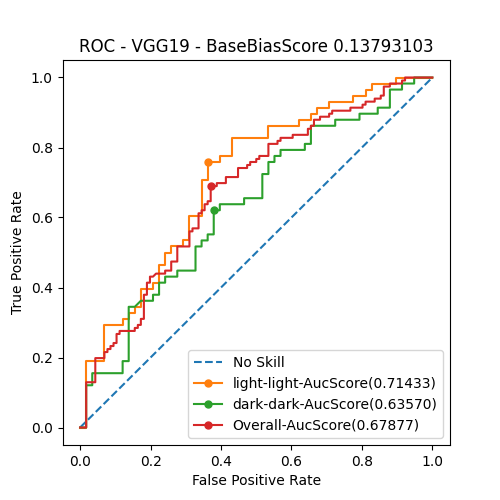
\includegraphics[width=0.9\linewidth]{latex/images/VGG19.png}}
    \caption{VGG19 ROC and Bias Score.}
    \label{vgg19_roc}
\end{figure}

\begin{figure}[htbp]
    \centerline{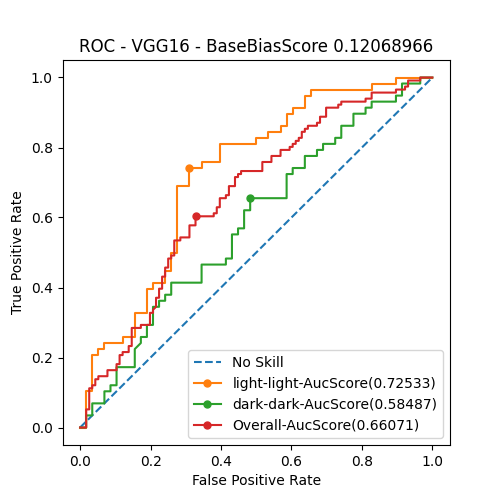
\includegraphics[width=0.9\linewidth]{latex/images/VGG16.png}}
    \caption{VGG16 ROC and Bias Score.}
    \label{vgg16_roc}
\end{figure}

\subsubsection{Bias/Performance trade-off}
Though we will not inherently be focusing on model performance, we will leverage this measurement to track the side effects of our hyper-parameters tuning.
This is the trade-off between bias reduction and facial verification performance, where a higher BPC means, bias reduction but low face verification drop while a lower BPC means the opposite (bias reduction with high facial verification performance reduction).

Utilizing Bias-Performance Characteristic (BPC) as an evaluation metric allows us to finely balance the trade-offs between reducing bias and maintaining high verification performance in facial recognition systems. This metric is crucial for our analysis as it ensures that while we aim to study the effect of their hyper-parameters tuning on bias, we do not inadvertently compromise the system's overall effectiveness. It guides our tuning process by quantifying the impact of changes on both bias reduction and facial recognition accuracy, enabling informed study on the achieved results.

\begin{equation}
    {BPC^{(F)}=\frac{Bias^{(F)}-Bias_{deb}^{(F)}}{Bias^{(F)}}}
\end{equation}

Where $Bias^{(F)}$ refer to the overall Bias obtained by original features and the corresponding bias at FPR of F. $Bias_{deb}^{(F)}$ denote their de-biased counterparts. 

\subsubsection{Accuracy}
Even though our primary focus is not on accuracy, we deemed this measurement metric as crucial to guide our fine-tuning process indicating the overall model performance as a baseline metric. It ensures that we can understand the significant impact of any changes made to address bias on a model's ability to correctly classify facial expressions.
Furthermore, monitoring accuracy can help identify if the model is over-fitting or under-fitting while we’re fine-tuning it.

\subsubsection{Visualization}
We used Grad-CAM (Gradient-weighted Class Activation Mapping) heat map visualization to visualize the region of an image that are important for predictions from the last layer of CNN. This help us to understand which facial features the model is focusing on for face identification or verification. This is relevant for our analysis of bias as it can reveal if the model is relying on features that are not evenly distributed across different demographic(racial) groups, potentially leading to bias prediction.

\begin{figure}
    \centerline{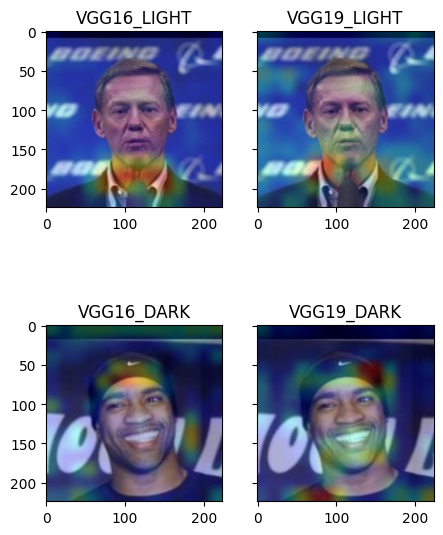
\includegraphics[width=0.8\linewidth]{latex/images/heatmap.png}}
    \caption{Grad-CAM heat maps of prediction focus regions.}
    \label{grad_cam}
\end{figure}

\subsection{Dataset}
\subsubsection{Training Dataset}
For the purpose of model training, we will be utilizing the FairFace Dataset\cite{karkkainen2021fairface}. This dataset contains 108,501 images and is balanced on race. Seven races are defined White, Black, Indian, East Asian, Southeast Asian, Middle East, and Latino. Images were collected from the YFCC-100M Flickr dataset\cite{thomee2016yfcc100m}.

\begin{figure}
    \centerline{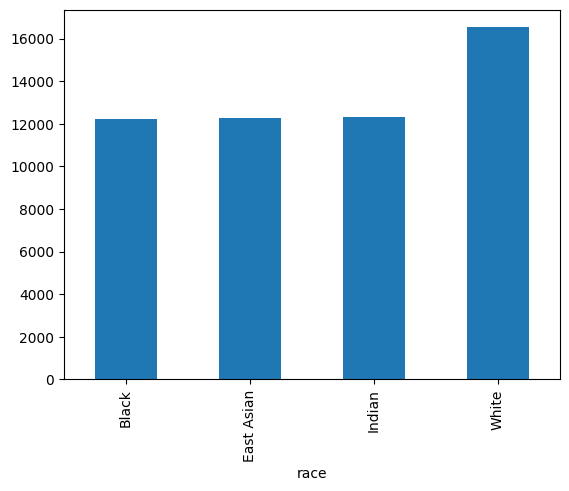
\includegraphics[width=0.8\linewidth]{latex/images/fairFaceOriginalDistribution.png}}
    \caption{Distribution of races in the FairFace training dataset.}
    \label{racial_distribution}
\end{figure}

\subsubsection{Binarization / Regrouping of the training dataset}
For ease of calculations and testing, we opted to follow in similar steps to\cite{dhar2022distill} in which we combine and binarize the dataset. Regrouping the FairFace\cite{karkkainen2021fairface} data set into two skin tone categories Light (‘White’ $\cup$ ‘East Asian’) and Dark (‘Indian’ $\cup$ ‘Black’). As \cite{dhar2022distill} mentions the skin label is not perfectly correlated with race, but it does have a high correlation nonetheless. 

\begin{figure}
    \centerline{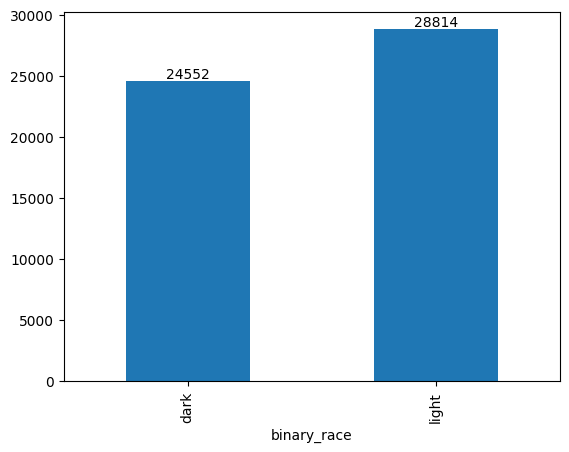
\includegraphics[width=0.8\linewidth]{latex/images/RegroupDistributionFairFace.png}}
    \caption{Dataset distribution after data binarization.}
    \label{binarized_data}
\end{figure}

The training data has 28,814 instances of ‘light’ and 24,552 of ‘dark’, which means we have an imbalance in our dataset. We will utilize random under-sampling to delete instances from the majority class ‘light’. For our study 24,552 instances per class should be sufficient to study the effect of hyper parameters on bias.

\section{Results and Conclusion}
\subsection{Limitations}
\subsubsection{Restricted Variation Study}
Our research primarily focuses on a limited subset of hyper-parameters, due to the complexity and extensive computational resources required for a broader analysis. By concentrating on key hyper-parameters, we aim to provide depth rather than breadth in our investigation. This strategic limitation allows for detailed exploration within the selected parameters but restricts our ability to generalize findings across a wider range of hyper-parameter configurations.
\subsubsection{Binarization of Racial Categories}
The decision to binarize racial categories into 'light' and 'dark' groups is driven by statistical considerations. This simplification facilitates a clearer analysis of bias and performance discrepancies between these two broadly categorized groups. However, this approach may overlook nuances and intra-group variations that could significantly impact model performance and bias. The reduction of racial diversity into binary categories is a pragmatic choice to manage complexity but may limit the granularity and applicability of our findings.
\subsubsection{Time Constraints}
The timeline of the research project has necessitated certain compromises in terms of the breadth and depth of the investigation. Extensive hyper-parameter tuning and larger-scale testing methodologies were curtailed to meet project deadlines. As a result, some potentially influential factors and interactions may not have been thoroughly explored.
\subsubsection{Computational Resource Limitations}
The availability of processing power is a significant constraint, particularly for deep learning models that require substantial computational resources. This limitation influenced our choice of models and the extent of hyper-parameter tuning feasible within our study, potentially restricting the robustness and variability of our experiments.









% \subsection{Maintaining the Integrity of the Specifications}

% The IEEEtran class file is used to format your paper and style the text. All margins, 
% column widths, line spaces, and text fonts are prescribed; please do not 
% alter them. You may note peculiarities. For example, the head margin
% measures proportionately more than is customary. This measurement 
% and others are deliberate, using specifications that anticipate your paper 
% as one part of the entire proceedings, and not as an independent document. 
% Please do not revise any of the current designations.

% \section{Prepare Your Paper Before Styling}
% Before you begin to format your paper, first write and save the content as a 
% separate text file. Complete all content and organizational editing before 
% formatting. Please note sections \ref{AA}--\ref{SCM} below for more information on 
% proofreading, spelling and grammar.

% Keep your text and graphic files separate until after the text has been 
% formatted and styled. Do not number text heads---{\LaTeX} will do that 
% for you.

% \subsection{Abbreviations and Acronyms}\label{AA}
% Define abbreviations and acronyms the first time they are used in the text, 
% even after they have been defined in the abstract. Abbreviations such as 
% IEEE, SI, MKS, CGS, ac, dc, and rms do not have to be defined. Do not use 
% abbreviations in the title or heads unless they are unavoidable.

% \subsection{Units}
% \begin{itemize}
% \item Use either SI (MKS) or CGS as primary units. (SI units are encouraged.) English units may be used as secondary units (in parentheses). An exception would be the use of English units as identifiers in trade, such as ``3.5-inch disk drive''.
% \item Avoid combining SI and CGS units, such as current in amperes and magnetic field in oersteds. This often leads to confusion because equations do not balance dimensionally. If you must use mixed units, clearly state the units for each quantity that you use in an equation.
% \item Do not mix complete spellings and abbreviations of units: ``Wb/m\textsuperscript{2}'' or ``webers per square meter'', not ``webers/m\textsuperscript{2}''. Spell out units when they appear in text: ``. . . a few henries'', not ``. . . a few H''.
% \item Use a zero before decimal points: ``0.25'', not ``.25''. Use ``cm\textsuperscript{3}'', not ``cc''.)
% \end{itemize}

% \subsection{Equations}
% Number equations consecutively. To make your 
% equations more compact, you may use the solidus (~/~), the exp function, or 
% appropriate exponents. Italicize Roman symbols for quantities and variables, 
% but not Greek symbols. Use a long dash rather than a hyphen for a minus 
% sign. Punctuate equations with commas or periods when they are part of a 
% sentence, as in:
% \begin{equation}
% a+b=\gamma\label{eq}
% \end{equation}

% Be sure that the 
% symbols in your equation have been defined before or immediately following 
% the equation. Use ``\eqref{eq}'', not ``Eq.~\eqref{eq}'' or ``equation \eqref{eq}'', except at 
% the beginning of a sentence: ``Equation \eqref{eq} is . . .''

% \subsection{\LaTeX-Specific Advice}

% Please use ``soft'' (e.g., \verb|\eqref{Eq}|) cross references instead
% of ``hard'' references (e.g., \verb|(1)|). That will make it possible
% to combine sections, add equations, or change the order of figures or
% citations without having to go through the file line by line.

% Please don't use the \verb|{eqnarray}| equation environment. Use
% \verb|{align}| or \verb|{IEEEeqnarray}| instead. The \verb|{eqnarray}|
% environment leaves unsightly spaces around relation symbols.

% Please note that the \verb|{subequations}| environment in {\LaTeX}
% will increment the main equation counter even when there are no
% equation numbers displayed. If you forget that, you might write an
% article in which the equation numbers skip from (17) to (20), causing
% the copy editors to wonder if you've discovered a new method of
% counting.

% {\LaTeX} can't read your mind. If you assign the same label to a
% subsubsection and a table, you might find that Table I has been cross
% referenced as Table IV-B3. 

% {\LaTeX} does not have precognitive abilities. If you put a
% \verb|\label| command before the command that updates the counter it's
% supposed to be using, the label will pick up the last counter to be
% cross referenced instead. In particular, a \verb|\label| command
% should not go before the caption of a figure or a table.

% Do not use \verb|\nonumber| inside the \verb|{array}| environment. It
% will not stop equation numbers inside \verb|{array}| (there won't be
% any anyway) and it might stop a wanted equation number in the
% surrounding equation.

% \subsection{Some Common Mistakes}\label{SCM}
% \begin{itemize}
% \item The word ``data'' is plural, not singular.
% \item The subscript for the permeability of vacuum $\mu_{0}$, and other common scientific constants, is zero with subscript formatting, not a lowercase letter ``o''.
% \item In American English, commas, semicolons, periods, question and exclamation marks are located within quotation marks only when a complete thought or name is cited, such as a title or full quotation. When quotation marks are used, instead of a bold or italic typeface, to highlight a word or phrase, punctuation should appear outside of the quotation marks. A parenthetical phrase or statement at the end of a sentence is punctuated outside of the closing parenthesis (like this). (A parenthetical sentence is punctuated within the parentheses.)
% \item A graph within a graph is an ``inset'', not an ``insert''. The word alternatively is preferred to the word ``alternately'' (unless you really mean something that alternates).
% \item Do not use the word ``essentially'' to mean ``approximately'' or ``effectively''.
% \item In your paper title, if the words ``that uses'' can accurately replace the word ``using'', capitalize the ``u''; if not, keep using lower-cased.
% \item Be aware of the different meanings of the homophones ``affect'' and ``effect'', ``complement'' and ``compliment'', ``discreet'' and ``discrete'', ``principal'' and ``principle''.
% \item Do not confuse ``imply'' and ``infer''.
% \item The prefix ``non'' is not a word; it should be joined to the word it modifies, usually without a hyphen.
% \item There is no period after the ``et'' in the Latin abbreviation ``et al.''.
% \item The abbreviation ``i.e.'' means ``that is'', and the abbreviation ``e.g.'' means ``for example''.
% \end{itemize}
% An excellent style manual for science writers is \cite{b7}.

% \subsection{Authors and Affiliations}
% \textbf{The class file is designed for, but not limited to, six authors.} A 
% minimum of one author is required for all conference articles. Author names 
% should be listed starting from left to right and then moving down to the 
% next line. This is the author sequence that will be used in future citations 
% and by indexing services. Names should not be listed in columns nor group by 
% affiliation. Please keep your affiliations as succinct as possible (for 
% example, do not differentiate among departments of the same organization).

% \subsection{Identify the Headings}
% Headings, or heads, are organizational devices that guide the reader through 
% your paper. There are two types: component heads and text heads.

% Component heads identify the different components of your paper and are not 
% topically subordinate to each other. Examples include Acknowledgments and 
% References and, for these, the correct style to use is ``Heading 5''. Use 
% ``figure caption'' for your Figure captions, and ``table head'' for your 
% table title. Run-in heads, such as ``Abstract'', will require you to apply a 
% style (in this case, italic) in addition to the style provided by the drop 
% down menu to differentiate the head from the text.

% Text heads organize the topics on a relational, hierarchical basis. For 
% example, the paper title is the primary text head because all subsequent 
% material relates and elaborates on this one topic. If there are two or more 
% sub-topics, the next level head (uppercase Roman numerals) should be used 
% and, conversely, if there are not at least two sub-topics, then no subheads 
% should be introduced.

% \subsection{Figures and Tables}
% \paragraph{Positioning Figures and Tables} Place figures and tables at the top and 
% bottom of columns. Avoid placing them in the middle of columns. Large 
% figures and tables may span across both columns. Figure captions should be 
% below the figures; table heads should appear above the tables. Insert 
% figures and tables after they are cited in the text. Use the abbreviation 
% ``Fig.~\ref{fig}'', even at the beginning of a sentence.

% \begin{table}[htbp]
% \caption{Table Type Styles}
% \begin{center}
% \begin{tabular}{|c|c|c|c|}
% \hline
% \textbf{Table}&\multicolumn{3}{|c|}{\textbf{Table Column Head}} \\
% \cline{2-4} 
% \textbf{Head} & \textbf{\textit{Table column subhead}}& \textbf{\textit{Subhead}}& \textbf{\textit{Subhead}} \\
% \hline
% copy& More table copy$^{\mathrm{a}}$& &  \\
% \hline
% \multicolumn{4}{l}{$^{\mathrm{a}}$Sample of a Table footnote.}
% \end{tabular}
% \label{tab1}
% \end{center}
% \end{table}

% \begin{figure}[htbp]
% \centerline{
\includegraphics{fig1.png}}
% \caption{Example of a figure caption.}
% \label{fig}
% \end{figure}

% Figure Labels: Use 8 point Times New Roman for Figure labels. Use words 
% rather than symbols or abbreviations when writing Figure axis labels to 
% avoid confusing the reader. As an example, write the quantity 
% ``Magnetization'', or ``Magnetization, M'', not just ``M''. If including 
% units in the label, present them within parentheses. Do not label axes only 
% with units. In the example, write ``Magnetization (A/m)'' or ``Magnetization 
% \{A[m(1)]\}'', not just ``A/m''. Do not label axes with a ratio of 
% quantities and units. For example, write ``Temperature (K)'', not 
% ``Temperature/K''.

% % \section*{Acknowledgment}

% The preferred spelling of the word ``acknowledgment'' in America is without 
% an ``e'' after the ``g''. Avoid the stilted expression ``one of us (R. B. 
% G.) thanks $\ldots$''. Instead, try ``R. B. G. thanks$\ldots$''. Put sponsor 
% acknowledgments in the unnumbered footnote on the first page.

% \section*{References}

% Please number citations consecutively within brackets \cite{b1}. The 
% sentence punctuation follows the bracket \cite{b2}. Refer simply to the reference 
% number, as in \cite{b3}---do not use ``Ref. \cite{b3}'' or ``reference \cite{b3}'' except at 
% the beginning of a sentence: ``Reference \cite{b3} was the first $\ldots$''

% Number footnotes separately in superscripts. Place the actual footnote at 
% the bottom of the column in which it was cited. Do not put footnotes in the 
% abstract or reference list. Use letters for table footnotes.

% Unless there are six authors or more give all authors' names; do not use 
% ``et al.''. Papers that have not been published, even if they have been 
% submitted for publication, should be cited as ``unpublished'' \cite{b4}. Papers 
% that have been accepted for publication should be cited as ``in press'' \cite{b5}. 
% Capitalize only the first word in a paper title, except for proper nouns and 
% element symbols.

% For papers published in translation journals, please give the English 
% citation first, followed by the original foreign-language citation \cite{b6}.

\bibliographystyle{IEEEtran}
\bibliography{Sources}

\end{document}
